\documentclass{book}

\usepackage[utf8]{inputenc}
\usepackage[T1]{fontenc}
\usepackage{lmodern}

\usepackage{pgfplots, pgfplotstable}
\pgfplotsset{compat=1.10}
\usepgfplotslibrary{units}
\usetikzlibrary{pgfplots.units}
\usetikzlibrary{positioning}

\def\samples{160}
\pgfmathdeclarefunction{examplepos}{1}{\pgfmathparse{e^(2.2*(#1)) - e^(10-5*(#1))}}
\pgfmathdeclarefunction{examplevel}{1}{\pgfmathparse{2.2*e^(2.2*(#1)) + 5*e^(10-5*(#1))}}
\pgfmathdeclarefunction{examplevel2}{1}{\pgfmathparse{e^(-((#1)-2)^2) + 2*e^(-((#1)-4)^2)}}

\usepackage{float,subcaption}
\usepackage[font=small,labelfont=bf]{caption}

\usepackage{tikz,tikz-3dplot}
\usetikzlibrary{calc,intersections}
\tikzset{point/.style={circle,fill,inner sep=1pt,label=above:{$\posit{#1}$}}}
\tikzset{boint/.style={circle,fill,inner sep=1pt,label=below:{$\posit{#1}$}}}
\tikzset{loint/.style={circle,fill,inner sep=1pt,label=left :{$\posit{#1}$}}}
\tikzset{roint/.style={circle,fill,inner sep=1pt,label=right:{$\posit{#1}$}}}

% set up spherical coordinates
\tdplotsetmaincoords{60}{110}

% inspired from http://tex.stackexchange.com/questions/38818/best-way-to-denote-an-angle-in-tikz/55555#55555
\newcommand\markangle[6][none]{% [color] {X} {origin} {Y} {mark} {radius}
	\begin{scope}
	\clip (#2.center) -- (#3.center) -- (#4.center);
	\draw[black,fill=#1,fill opacity=0.5,name path=markangleC] (#3) circle (#6);
	\end{scope}

	% middle calculation
	\path[name path=markangleL1] (#3) -- (#2);
	\path[name path=markangleL2] (#3) -- (#4);
	\path[name intersections={of=markangleL1 and markangleC, by={markangleX1}},
	      name intersections={of=markangleL2 and markangleC, by={markangleX2}}]
	      (markangleX1) -- (markangleX2) coordinate[pos=.5] (middle);

	% bissectrice definition
	\path[name path=markangleB] (#3) -- (barycentric cs:#3=-1,middle=1.2);

	% put mark
	\path[name intersections={of=markangleB and markangleC, by={markanglemiddleArc}}]
		(#3) -- (markanglemiddleArc) node[pos=1.5] {\angle{#5}};
}
% inspired from http://tex.stackexchange.com/questions/123158/tikz-using-the-ellipse-command-with-a-start-and-end-angle-instead-of-an-arc/123187#123187
\tikzset{partial ellipse/.style args={#1:#2:#3}{
	insert path={+ (#1:#3) arc (#1:#2:#3)}
}}
\newcommand{\orbit}[6][]{% options, focus, apoapsis, periapsis, start angle, end angle
\begin{scope}[shift={(#2)}]
	\pgfmathsetmacro{\orbitLap}{(#3)}
	\pgfmathsetmacro{\orbitLpe}{(#4)}
	\pgfmathsetmacro{\orbitLa}{(\orbitLap+\orbitLpe)/2}
	\pgfmathsetmacro{\orbitLb}{sqrt(\orbitLap*\orbitLpe)}
	\pgfmathsetmacro{\orbitLe}{(\orbitLap-\orbitLpe)/(\orbitLap+\orbitLpe)}
	\pgfmathsetmacro{\orbitLf}{\orbitLa*\orbitLe}
	\draw[-latex,thick,#1]
	plot[domain=#5:#6,samples=\samples]
		({\x}:{\orbitLa*(1-\orbitLe*\orbitLe)/(1-\orbitLe*cos(\x))});
\end{scope}
}
\newcommand{\orbitpoint}[7][]{% options, focus, apoapsis, periapsis, angle, name, label
\begin{scope}[shift={(#2)}]
	\pgfmathsetmacro{\orbitpointLap}{(#3)}
	\pgfmathsetmacro{\orbitpointLpe}{(#4)}
	\pgfmathsetmacro{\orbitpointLa}{(\orbitpointLap+\orbitpointLpe)/2}
	\pgfmathsetmacro{\orbitpointLb}{sqrt(\orbitpointLap*\orbitpointLpe)}
	\pgfmathsetmacro{\orbitpointLe}{(\orbitpointLap-\orbitpointLpe)/(\orbitpointLap+\orbitpointLpe)}
	\pgfmathsetmacro{\orbitpointLf}{\orbitpointLa*\orbitpointLe}
	\pgfmathsetmacro{\orbitpointLang}{#5}
	\pgfmathsetmacro{\orbitpointLrad}{\orbitpointLa*(1-\orbitpointLe*\orbitpointLe)/(1-\orbitpointLe*cos(\orbitpointLang))}
	\node[-latex,thick,#1] (#6) at (\orbitpointLang:\orbitpointLrad) {#7};
\end{scope}
}
\newcommand{\horbit}[5][]{% options, focus, periapsis, eccentricity, domain
	\draw[-latex,thick,#1] let \p1=(#2) in \pgfextra{
		\pgfmathsetmacro{\horbitLap}{#3}
		\pgfmathsetmacro{\horbitLe}{#4}
		\pgfmathsetmacro{\horbitLa}{\horbitLap/abs(\horbitLe-1)}
		\pgfmathsetmacro{\horbitLb}{(\horbitLa*sqrt(abs(\horbitLe*\horbitLe-1))}
		\pgfmathsetmacro{\Ox}{\x1/1cm}
		\pgfmathsetmacro{\Oy}{\y1/1cm}
	}
	plot[domain=-#5:#5,samples=\samples]
		({\Ox - \horbitLa - \horbitLap + \horbitLa*cosh(\x)},{\Oy + \horbitLb*sinh(\x)});
}

\raggedbottom

\usepackage[colorlinks,linkcolor=blue]{hyperref}

%\renewcommand{\thechapter}   {\Roman {chapter}}
%\renewcommand{\thesection}   {\arabic{section}}
%\renewcommand{\thesubsection}{\arabic{section}.\arabic{subsection}}

\usepackage{fancyhdr}
\renewcommand{\headrulewidth}{0pt}
\renewcommand{\footrulewidth}{0.4pt}
\pagestyle{fancy}
\fancyhf{}
\fancyfoot[RE]{\leftmark}
\fancyfoot[LE,RO]{\thepage}
\fancypagestyle{plain}{
\renewcommand{\footrulewidth}{0pt}
\fancyhf{}
}

\definecolor{quotemark}{gray}{0.7}
\newcommand{\chaptquote}[2]{
\begin{flushleft}
{\bfseries\Huge\color{quotemark}``}
#2
\put(5,-15){\bfseries\Huge\color{quotemark}''}
\end{flushleft}
\vspace*{-1.5em}\hfill -- #1\vspace{2em}
}

\setlength{\marginparwidth}{0mm}

% information and warning blocks
% inspired http://tex.stackexchange.com/questions/53245/pretty-formattings-for-warning-and-info-blocks
\usepackage{mdframed}
\newenvironment{important}[1][]{\begin{mdframed}[%
	backgroundcolor={red!15}, hidealllines=true,
	skipabove=1.0\baselineskip, #1
]%
	\makebox[0pt]{\smash{% ignore width and height
		\fontsize{32pt}{32pt}\selectfont% size
		\hspace*{-19pt}\raisebox{-2pt}{% position
			\color{red!70!black}\sffamily\bfseries !%
		}%
	}}%
}{\end{mdframed}}
\newenvironment{remark}[1][]{\begin{mdframed}[%
	backgroundcolor={green!15}, hidealllines=true,
	skipabove=1.0\baselineskip, #1
]%
	\makebox[0pt]{\smash{% ignore width and height
		\fontsize{32pt}{32pt}\selectfont% size
		\hspace*{-19pt}\raisebox{-2pt}{% position
			\color{green!70!black}\sffamily\bfseries ?%
		}%
	}}%
}{\end{mdframed}}

% back cover
\usepackage[absolute]{textpos}

% chapter banners
\usepackage{wallpaper}
% inspired from http://tex.stackexchange.com/questions/64061/creating-variables-with-index-using-counters/64082#64082
\newcommand\addindex[4][]{% ???, var name, index, value
	\csname#1def\expandafter\endcsname\csname #2#3\endcsname{#4}%
}
\newcounter{BannerCount}
\setcounter{BannerCount}{0}
\newcommand\addbanner[1]{
	\stepcounter{BannerCount}
	\expandafter\addindex{banners}{\theBannerCount}{#1}
}
\newcommand\banner{\ClearWallPaper\ULCornerWallPaper{1}{img/banners/\csname banners\thechapter\endcsname.jpg}}
\addbanner{minmus}
\addbanner{gilly}
\addbanner{eve}
\addbanner{duna}
\addbanner{ike}
\addbanner{laythe}
\addbanner{jool}
\addbanner{pol}

% automatically scale graphics
\usepackage[export]{adjustbox} % also load graphicx
\let\Oldincludegraphics\includegraphics
\renewcommand{\includegraphics}[2][]{\Oldincludegraphics[max width=\textwidth,#1]{#2}}


\usepackage{mathtools, esint}
\newcommand\eqtag[1]{\addtocounter{equation}{1}\tag{\theequation}\label{#1}}
\renewcommand{\d}{\mathrm{d}}
\newcommand{\dt}{\d t}
\newcommand{\dm}{\d m}
% inspired from http://tex.stackexchange.com/questions/20643/diagonal-strikeout-starting-too-low-and-ending-too-high
\newcommand{\strike}[2][black]{\tikz[baseline=(box.base)]{
	\node[inner sep=0pt,outer sep=0pt] (box) {$#2$};
	\draw[#1] (box.south west) -- (box.north east);
}}


\def\samples{160}
\usepackage{blindtext}
%\includeonly{mechanics}

\begin{document}
\usetikzlibrary{3d}
\begin{titlepage}

\tikzifexternalizing{}{
% inspired from http://www.latex-community.org/forum/viewtopic.php?p=4950&sid=f71d94b93af6e784fa70c5e983e083ba#p4950
\thispagestyle{empty}
\begin{textblock*}{\paperwidth}(0mm,0mm)
\noindent\includegraphics[height=\paperheight]{img/front.jpg}
\end{textblock*}
}

\tikzifexternalizing{}{
\begin{textblock*}{\paperwidth}(0mm,2mm){
\centering \color{title}
\fontsize{1cm}{1em}\selectfont
Advised Introduction to \\
\fontsize{2cm}{1em}\selectfont
\textbf{Rocket Science}
\fontsize{0.5cm}{1em}\selectfont
(Ignoring Collisions) \\
\fontsize{1cm}{1em}\selectfont
for Kerbals \\
}\end{textblock*}
}

\mbox{}
\newpage
\end{titlepage}

\setcounter{tocdepth}{1}

% inspired from http://tex.stackexchange.com/questions/139289/removing-extra-page-before-and-after-tableofcontents/139334#139334
\begingroup
\let\cleardoublepage\clearpage
\tableofcontents
\endgroup

\chapter*{Introduction}
% inspired from http://stackoverflow.com/questions/2488681/latex-unnumbered-section-in-header-of-document/2492571#2492571 
\markboth{\MakeUppercase{Introduction}}{}
%\addcontentsline{toc}{chapter}{Introduction}

\chaptquote{Neil Armstrong}{That's one small step for a man, one giant leap for mankind.}

Kerbal Space Program \cite{ksp} is a rocket simulation game; it lets
you build, launch and pilot a rocket to put up satellites, send probes,
land rovers, and have Kerbals do SCIENCE.

\begin{figure}[H]
\includegraphics[width=\textwidth]{img/xkcd1356.png}
\caption{
	Mouseover text reads ”To be fair, my job at NASA was working
	on robots and didn't actually involve any orbital mechanics. The
	small positive slope over that period is because it turns out
	that if you hang around at NASA, you get in a lot of conversations
	about space.” \cite{xkcd1356}
}
\end{figure}

A big advantage a KSP player has over actual rocket crafters is that she
can have rockets exploding without having to worry about consequences.
Half the fun of the game comes from finding out why your next rocket
will fail; thus, I urge you roll rockets to the launchpad early and not
bother thinking of every little thing that could go wrong.

AIRSICK will not cover the initiation to the game, since the interface is
specific to the game and prone to change. The game offers an intuitive
way to assemble rockets and has a handy interface to control the
flight. Rather, it will expose, explain and detail real principles of
physics that the game mimics. This information can be read simply for
curiosity, or can serve to design more precise launches in the game. When
possible, example values will be taken from reality or KSP.

\begin{remark}
KSP is a propietary software. You can play the demo for free, but will
be limited to an older version with only a few parts available for
building. The demo is way harder and the complete game way richer.
\end{remark}

\begin{important}
This document is intended to provide information both for beginners and
actual physicists. The first few chapters are an introduction to the
elementary concepts used within this book. In every chapters accurate
derivations and complete proofs are developed wherevever needed. If you
are not interested in the specifics of a demonstration or have already
some knowledge of basics physics, feel free to skip irrelevant parts.
\end{important}



\section*{Credits}

This document makes extensive use of pictures, diagrams and various
illustrations. Most figures were generated with the file from \LaTeX
using the Tikz package. When an external image was included as a figure,
a reference to the source is linked in the caption (e.g. \cite{xkcd1356}).

The image on the front cover \cite{3kerbalmun} and the chapter banners
\cite{banners} are KSP fan arts; the last illustration is a wallpaper
available on the official website of the game \cite{ksp}.

\chapter{Basics}
\banner
\chaptquote{Carl Sagan}{
	Imagination will often carry us to worlds that never were. But
	without it we go nowhere.
}



\section{Units}


\subsection{Dimensions}

There exist different units for each kind of measure (e.g. \dist{distance}
in \dist{meters}, \dist{feet}, etc. To avoid confusion, we agreed on which
units should be prefered; they are called SI Units (for \emph{Système
International}, International System).

\begin{figure}[H]
\centering
\begin{tabular}{l|l|l}
Dimension        & SI unit       & Other units                   \\ \hline
\angle{angle}    & radian (-)    & turn (-), degree ($^{\circ}$) \\ \hline
\delay{duration} & second (s)    & hour (h), day (d), year (y)   \\ \hline
\dist {distance} & meter (m)     & feet, miles, light-year (ly)  \\ \hline
\speed{speed}    & m/s           & km/h, knot                    \\ \hline
\mass {mass}     & kilogram (kg) & ton, pound                    \\ \hline
       pressure  & pascal (Pa)   & atmosphere (atm)              \\ \hline
\end{tabular}
\caption{In this context, a dimension is a type of measure.}
\end{figure}

\begin{remark}
A \dist{light} year is the distance that a particle of light can travel
in a \delay{year} of time. For comparison, it takes light a little more
than \delay{eight minutes} (\delay{8~min}) to get from the Sun to the
Earth, meaning that the Sun is \dist{8~light-minutes} away from the
Earth. Kerbin is about \dist{45~light-seconds} away from Kerbol.
\end{remark}



\subsection{Prefixes}

We are used to refer to \dist{10,000 meters} (\dist{m}) as \dist{10
kilometers} (\dist{km}). “kilo-” is a prefix meaning “thoussand”;
it is the most used prefix but others exist:

\begin{figure}[H]
\centering
\begin{tabular}{l|l|l|l}
kilo- (k-) & mega- (M-) & giga- (G-) & tera- (T-) \\
\hline
$10^3$     & $10^6$     & $10^9$     & $10^{12}$  \\
\end{tabular}
\caption{Common prefixes}
\end{figure}

\begin{remark}
There are also prefixes to decrease the value of an unit:

\begin{figure}[H]
\centering
\begin{tabular}{l|l|l|l}
milli- (m-) & micro- ($\mu$-) & nano- (n-) & pico- (p-) \\
\hline
$10^{-3}$   & $10^{-6}$       & $10^{-9}$  & $10^{-12}$ \\
\end{tabular}
\caption{Smaller prefixes}
\end{figure}
\end{remark}


\subsection{Conversion}

We sometimes need to switch the unit used for a measure. For example,
let us convert $\speed{50~km/h}$ to SI units. We know that $\dist{km}
= \dist{1000~m}$ and $\delay{h} = \delay{3600~s}$ so:

\[
\speed{50~km/h}
= 50 (\dist{1000~m})/(\delay{3600~s})
= 50 \times 1000 / 3600 \speed{m/s}
= \speed{14~m/s}
\]

This particular example shows how easy it is to include units in
computations. As we will see below, having the units is useful when
considering more complex expressions.


\subsection{Addition (and substraction)}

An addition can only be done with the same kind of measure (e.g. a
distance can only be summed with another distance). This is seems obvious,
but simply checking that the values that are being some are actually of
the same kind can help locate errors early and save tremendous amounts
of time. Now, consider the following operation:

\[
\dist{x} = \dist{2~ly} + \dist{4,730.3~Tm}
\]

We do not know how to sum arbitrary units (for instance \dist{m}
with \mass{kg}). However, we do know that that $\dist{ly} =
\dist{9.4607~Tm}$. Thus, we can replace it in the expression:

\begin{align*}
\dist{x}
&= 2 \times \dist{ly} + \dist{4,730.3~Tm} \\
&= 2 \times \dist{9.4607~Tm} + \dist{4,730.3~Tm} \\
&= (18.92146 + 4,730.3) \dist{Tm} \\
&= \dist{23.6518~Tm}
\end{align*}

Conversly, we could also have said that $\dist{Tm} = \dist{1/9.4607~ly}$
and then:

\begin{align*}
\dist{x}
&= \dist{2~ly} + \dist{4,730.3~Tm} \\
&= \dist{2~ly} + (4,730.3 / 9.4607) \dist{ly} \\
&= (2 + 0.5) \dist{ly} \\
&= \dist{2.5~ly}
\end{align*}

Of course, the two ways are equivalent and we can check that
$\dist{2.5~ly} = \dist{23.6518~Tm}$.


\subsection{Multiplication (and division)}

We can create new units pretty easily. For example, if some object
travels a distance $\dist{d} = \dist{15~m}$ in a duration $\delay{t}
= \delay{3~s}$, we can define the velocity $\speed{v} = \dist{d} /
\delay{t} = \dist{15~m} / \delay{3~s} = \speed{5~m/s}$. Conversely,
assume the object has traveled at a velocity $\speed{50~km/h}$ for a
duration $\delay{30~s}$; then, the distance it has gone through is:

\[
\dist{d}
= \speed{v} \times \delay{t}
= (\speed{50~km/h}) \times (\delay{30~s})
= 14~\speed{m/s} \times 30~\delay{s}
= (14 \times 30) (\dist{m}/\strike[red]{\delay{s}} \times \strike[red]{\delay{s}})
= \dist{417~m}
\]

By doing the operations on both the numerical values and the units,
we know what our result is: in this case, it's a distance, and it is
expressed in meters.



\section{Functions}

\begin{figure}[H]
\centering
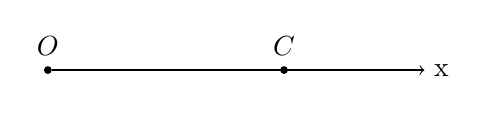
\begin{tikzpicture}[->]
\node[point=O] (O) at (0,0) {};
\node          (E) at (5,0) {x};
\node[point=C] (C) at (3,0) {};
\draw (O) -> (E);
\end{tikzpicture}
\caption{$\posit{C}$ is moving towards the right at speed $\speed{v}$}
\end{figure}

Let us consider a car $\posit{C}$ moving along a straight road at a
speed of $\speed{v}$ (e.g. $\speed{50~km/h}$). The position of the car,
$\posit{C}$, can be determined by the distance from $\posit{C}$ to an
arbitrary fix point $\posit{O}$ (the \textbf{origin}). We will note this
distance $\dist{x}$ and we have thus $\dist{x} = \dist{OC}$.

Say we are interested in the variations of the position of the car as
time changes and say write the current time $\delay{t}$ as the delay since
the car was at the origin ($\posit{C} = \posit{O}$).

In other words, we are interested in $\dist{x}$ as a \textbf{function}
of $\delay{t}$. After some time $\delay{t}$ has passed (e.g. $\delay{t}
= delay{10~s}$), we know that $\dist{x} = \speed{v} \times \delay{t}$. We
write it:

\[
\dist{x}(\delay{t}) = \speed{v} \times \delay{t}
\]

This notation gives us a general formula to compute $\dist{x}$ for any
given value of $\delay{t}$. For example:

\[
\dist{x}(\delay{1~h})
= \speed{50~km/h} \times \delay{1~h}
= \dist{50~km}
\]

As another example, it is known that the intensity of the light emitted by a star decreases proportionnaly to the square of the distance to the star. This can be written as:

\[
L(\dist{r}) = \frac C {\dist{r}^2}
\]

where $C$ is some \textbf{constant} value (i.e. independent from
$\dist{r}$) which is to be determined experimentally.



\section{Derivatives}


\subsection{Definition}

Assume we know the position $\dist{x}(\delay{t})$ of the car for any
instant $\delay{t}$ and we want to determine the velocity of the car at
a given instant $\delay{t_0}$.

\pgfmathdeclarefunction{examplepos}{1}{\pgfmathparse{e^(2.2*(#1)) - e^(10-5*(#1)) + 22024}}
\begin{figure}[H]
\centering
\begin{tikzpicture}
\begin{axis}[
	samples=\samples,
	domain=0:5,
	ticks=none,
	no markers,
	axis lines=left,
	xlabel=$\delay{t}$,
	ylabel=$\dist{x}$,
	legend pos=north west,
	clip=false,
]
\addplot{examplepos(x)};
\node[roint=A] (A) at (axis cs:4, {examplepos(4)}) {};
\node[boint={\delay{t_0}}] (t) at (A |- {axis cs:0,0}) {};
\node[loint={\dist{x}(\delay{t_0})}] (x) at (A -| {axis cs:0,0}) {};
\draw[dashed] (t) -- (A) -- (x);
\addlegendentry{$\dist{x}(\delay{t})$}
\end{axis}
\end{tikzpicture}
\caption{
	The horizontal axis represents the passage of time, the vertical
	axis the position. The blue line shows the current position of
	the current at every instant. We are interested in the instant
	$\delay{t_0}$; this is noted $\posit{A}$ on the graph.
}
\end{figure}

The velocity is a the \textbf{variation} of position through time. Thus,
to know how fast the car is going at time $\delay{t_0}$, we need to look
at the position of the car at two different instants. We already have
$\delay{t_0}$; let us also consider $\delay{t_0+h}$ for some arbitrary
value $\delay{h}$.

The difference in position between instants $\delay{t_0}$ and
$\delay{t_0+h}$ is thus $\dist{x}(\delay{t_0+h}) - \dist{x}(\delay{t_0})$;
a shorter notation for this is $\dist{\Delta x}(\delay{t_0})$. The
value $\delay{h}$ is not shown because we do not really care about
it. The Greek letter $\Delta$, for $d$, is generally used to denote a
\textbf{d}ifference (here, the difference in position).

Notice that, the bigger $\delay{h}$, the bigger we expect this difference
to be; to compensate for this, we will divide by how much time has passed,
which is to say $\delay{t_0+h} - \delay{t_0} = \delay{\Delta t_0})$:

\[
\frac {\dist{\Delta x}(\delay{t_0})} {\delay{\Delta t_0}}
\]

This value is the \textbf{mean velocity} from instant $\delay{t_0}$ to
instant $\delay{t_0+h}$. However, the mean velocity is a value that
only gives a general idea of the speed on some period of time. In this
duration, the \textbf{instant velocity} (actual speed) can very a lot
and the mean velocity would then be far off to these values.

\begin{figure}[H]
\centering
\begin{tikzpicture}
\begin{axis}[
	samples=\samples,
	domain=0:5,
	ticks=none,
	no markers,
	axis lines=left,
	xlabel=$\delay{t}$,
	ylabel=$\dist{x}$,
	legend pos=north west,
	clip=false,
]
\addplot{examplepos(x)};
\node[roint=A] (A) at (axis cs:4.0, {examplepos(4.0)}) {};
\node[roint=B] (B) at (axis cs:4.9, {examplepos(4.9)}) {};
\node[boint={\delay{t_0}}]   (t0) at (A |- {axis cs:0,0}) {};
\node[boint={\delay{t_0+h}}] (t1) at (B |- {axis cs:0,0}) {};
\node[loint={\dist{x}(\delay{t_0})}]   (x0) at (A -| {axis cs:0,0}) {};
\node[loint={\dist{x}(\delay{t_0+h})}] (x1) at (B -| {axis cs:0,0}) {};
\draw[dashed] (t0) -- (A) -- (x0);
\draw[dashed] (t1) -- (B) -- (x1);
\draw[color=red,shorten <=-2cm,shorten >=-1cm] (A) -- (B);
\addlegendentry{$\dist{x}(\delay{t})$}
\end{axis}
\end{tikzpicture}
\caption{
	We add a point $\posit{B}$ to the previous graph at time
	$\delay{t_0}+h$. The mean velocity from $\posit{A}$ to $\posit{B}$
	can be thought as the slope of the red line $(AB)$.
}
\end{figure}

Since
we expect the speed to not change a lot on short periods of time, a
natural solution is to consider the mean velocity over shorter durations.

\begin{figure}[H]
\centering
\foreach \i in {0,...,3}{
	\begin{subfigure}{0.4\textwidth}
	\begin{tikzpicture}[scale=0.5]
		\begin{axis}[
		samples=\samples,
		domain=0:5,
		ticks=none,
		no markers,
		axis lines=left,
		legend pos=north west,
		clip=false,
		]
	\addplot{examplepos(x)};
	\node[roint=A] (A) at (axis cs:4.0, {examplepos(4.0)}) {};
	\node[loint=B] (B) at (axis cs:{4.0+0.9/(2^\i)}, {examplepos(4.0+0.9/(2^\i))}) {};
	\draw[color=red,shorten <=-2cm,shorten >=-1cm] (A) -- (B);
	\end{axis}
	\end{tikzpicture}
	\end{subfigure}
}
\caption{
	The closer to $\posit{A}$ we pick $\posit{B}$, the best the red
	line matches the curve for velocity at $\posit{A}$.
}
\end{figure}

So, as we pick shorter and shorter durations $\delay{h}$, the value
$\delay{\Delta t_0}$ becomes smaller, but so does $\dist{\Delta
x}$. Often, we will notice that the mean velocity over $\delay{h}$
seems to becomes closer and closer to a particular value. Instead of
continuing to choose smaller and smaller values of $\delay{h}$, we will
pick this values and call it the \textbf{limit} of $\frac {\dist{\Delta
x}(\delay{t_0})} {\delay{\Delta t_0}}$ as $\delay{h}$ tends to $0$
(becomes smaller and smaller):

\[
\lim_{\delay{h} \to \delay{0}} \frac {\dist{\Delta x}(\delay{t_0})} {\delay{\Delta t_0}}
\]

The limit of such an expression is called the \textbf{derivative} of
$\posit{x}$ at $\delay{t_0}$. We have a shorter way to note this:

\[
\frac {\dist{\d x}(\delay{t_0})} {\delay{\dt}}
\]

We can then remark that we have actually defined the derivative for any
$\delay{t_0}$. Thus, we have a new function that let us evaluate the
velocity at any $\delay{t_0}$.

\[
\frac {\dist{\d x}} {\delay{\dt}}
\]

\begin{remark}
An even shorter notation is $\speed{\dot x}$. This notation is only used
for derivatives with respect to time.
\end{remark}


\subsection{Second derivative}

The velocity is the derivative of the position. As a function, it can
itself fluctuate and we can be interested in these variations. The
derivative of the velocity is the \textbf{acceleration}: $\accel{a} =
\accel{\dot v}$.

A shorter way of saying that the acceleration is the derivative of
\textit{the derivative of the position}, is to say that the acceleration
is the second derivative of the position: $\accel{a} = \accel{\ddot x}$.


\subsection{Formal derivation}

While we now have a way to compute the derivative of a function at a
given point, it is not accurate: while we do get a better approximation
by taking a smaller value for $h$, the result is still an approximation
and can sometimes stay far off.

Instead, we can look at the expressions to determine the exact value
for the limit. For instance, let us consider the function $f(x) = 12x$
and let us search for $\frac {\d f(x)} {\d x}$ for any given $x$. First:

\[
\frac {\Delta f(x)} {\Delta x}
= \frac {f(x+h) - f(x)} {(x+h) - x}
= \frac {12(x+h) - 12x} {h}
= \frac {12\strike[red]{h}} {\strike[red]{h}}
= 12
\]

We now look at the value $\frac {\Delta f(x)} {\Delta x}$ as $\Delta x$
gets small; in this case, it happens to always be $12$, and does not
depend on $\Delta x$. Thus, however small $\Delta x$, the value is
$12$, and:

\[
\frac {\d f(x)} {\d x}
= \lim_{h \to 0} \frac {\Delta f(x)} {\Delta x}
= 12
\]

That way, we know the exaxt value of derivative of $f$ in any point. Let
us take a second example with $g(x) = 7x^2$:

\[
\frac {\Delta g(x)} {\Delta x}
= \frac {7(x+h)^2 - 7x^2} {h}
= \frac {7(x^2 + 2xh + h^2) - 7x^2} {h}
= \frac {7x\strike[red]{h} + h^{\strike[red]{2}}} {\strike[red]{h}}
= 7x + h
\]

Here, the expression does depend on $h$. However, the smaller $h$ gets,
the less influence it has on the sum: the value is becoming closer and
closer to $7x$. Thus: $\frac {\d g(x)} {\d x} = 7x$.


\subsection{Derivation rules}

Now, what if we want to compute the derivative of $h(x) = 12x +
7x^2$? Of course, we could go through the same step as in the previous
part. However, we can notice that $h = f + g$ (this means that $h(x)
= f(x) + g(x)$ for all $x$'s). It turns out that it can be shown that
$\frac {\d} {\d x} (f+g) = \frac {\d} {\d x} f + \frac {\d} {\d x} g$
for any functions $f$ and $g$. Using this rule and knowing the derivative
of $f$ and $g$, we can derive:

\[
\frac {\d} {\d x} h(x)
= \frac {\d} {\d x} (f+g)(x)
= \frac {\d} {\d x} f(x) + \frac {\d} {\d x} g(x)
= 12 + 7x
\]

There are a few derivation rules that can help us determine the derivative
of complex functions easily.

\begin{figure}[H]
\begin{subfigure}{0.45\textwidth}
\begin{alignat*}{2}
& (\alpha f)'              &&= \alpha f' \\
& (f + g)'                 &&= f' + g' \\
& (f \times g)'            &&= f' \times g' + g' \times f \\
& \left(\frac f g\right)'  &&= \frac {f'g - g'f} {g^2} \\
& (f(g(x))'                &&= g'(x) \times f'(g(x))
\end{alignat*}
\caption{derivation rules}
\end{subfigure}
\begin{subfigure}{0.45\textwidth}
\begin{alignat*}{2}
& (x^n)'    &&= n x^{n-1}   \\
& (e^x)'    &&= e^x         \\
& (\ln x)'  &&= \frac 1 x \\
& (\cos x)' &&= -\sin x \\
& (\sin x)' &&=  \cos x
\end{alignat*}
\caption{common derivatives}
\end{subfigure}
\end{figure}



\section{Integrals}


\subsection{Concept}

Once more, consider the car on the road. We are given its speed
$\speed{\dot x}(\delay{t})$ through the time. Because we know how fast the
car was going at any single instant, we can deduce how much it traveled
from time $\delay{t_1}$ to $\delay{t_2}$ for example. The computation
of the position depending on the speed is
noted with the integral symbol (which just means sum of small elements):
\[
\int_{\delay{t_1}}^{\delay{t_2}} \speed{\dot x}(\delay{t}) \delay{\dt}
= \int_{\delay{t_1}}^{\delay{t_2}} \frac {\dist{\d x}} {\strike[red]{\delay{\dt}}} \strike[red]{\delay{\dt}}
= \sum_{\delay{t_1}}^{\delay{t_2}} \dist{\d x}
= \underbrace{
	\dist{x}(\delay{t_2}) - \dist{x}(\delay{t_1})
}_{[\dist{x}]_{\delay{t_1}}^{\delay{t_2}}}
\]


\subsection{Illustration}

For example, if $\speed{\dot x} = \accel{2~m/s^2} \times \delay{t}$, then:
\begin{align*}
\dist{x}(\delay{30~s}) - \dist{x}(\delay{0~s})
&= \int_{\delay{0}}^{\delay{30~s}} \accel{2~m/s^2} \times \delay{t} \delay{\dt} \\
&= \left(\int_{\delay{0})}^{\delay{30~s}} 2 \delay{t} \delay{\dt}\right) \accel{m/s^2} \\
&= [\delay{t}^2]_{\delay{0}}^{\delay{30~s}} \accel{m/s^2} \\
&= (900~s^2 - 0~s^2) \accel{m/s^2} \\
&= \dist{900~m}
\end{align*}

In particular, with we are given the additional information that $\posit{C}$
did start at $\posit{O}$, i.e.  $\dist{x}(\delay{0}) = \dist{0}$, then:
\[
\dist{x}(\delay{30~s}) = \dist{900~m}
\]


\subsection{Antiderivative}

More generally, in the previous example, we could write:
\[
\dist{x}(\delay{t}) - \dist{x}(\delay{0})
= \int_{\delay{0}}^{\delay{30~s}} \accel{2~m/s^2} \times \delay{t} \delay{\dt}
= \delay{t}^2 \accel{m/s^2}
\]

Another way to write it is:
\[
\dist{x}(\delay{t})
= t^2 \accel{m/s^2} + \dist{C}
\]
where $\dist{C} = \dist{x}(\delay{0})$ is a value independent of
$\delay{t}$ which depends on the \textbf{initial conditions} (e.g. the
position of the car at the initial instant). Each of the possible
expression of $\dist{x}$ (depending on $\dist{C}$) is a primitive of
$\speed{\dot x}$.



\section{Differential equations}


\subsection{Definition}

A differential equation is an equation whose unknown is a function in
which a derivative of this function appears. For example:
\[
\frac {\d f} {\d x} = 3x^2
\]

This is a differential equation and we already know how to solve it
(find the expression of $f$). Here, $f(x) = x^3 + C$ (there are several
possible solutions).


\subsection{Exponential}

The exponential function is defined as $f(x) = e^x$ where $e$ is a
mathematical constant whose value is about $2.718$. It was picked so that:
\[
\frac {\d f} {\d x} = f
\]

In other words:
\[
\frac {\d} {\d x} (e^x) = e^x
\]

\begin{remark}
If we define $f(x) = e^{g(x)}$ instead, derivation rules
gives us:
\[
\frac {\d f(x)} {\d x}
= g'(x) e^{g(x)}
\]
so that $\frac {\d f} {\d x} = g' f$.
\end{remark}


\subsection{First order}

Now, consider the following equation:
\[
\frac {\d f} {\d x} = f
\]

We already know that $f(x) = e^x$ is a solution; however, so is $f(x) =
2 e^x$. Actually, the set of solutions to this equation is the functions
$f(x) = C e^x$ where $C$ is any constant value.

The remark we made before tell us how to solve a differential equation
of the form:
\[
\frac {\d f} {\d x} = h f
\]
where $h$ is also a function. We just need to find $g$ such that $g' =
h$, i.e. the solutions are:

\[
f(x) = C e^{\int_0^x h(x) \d x}
\]


\section{Geometric integrals}

Circle circumference:
\begin{align*}
\dist{d}
&= \oint_C \dist{\d s}
\\
&= \int_{\angle{0}}^{\angle{2\pi}} \dist{R} \angle{\d \theta}
\\
&= \dist{R} \left[ \theta \right]_{\angle{0}}^{\angle{2\pi}}
\\
&= 2\pi \dist{R}
\\
\end{align*}

Disk area:
\begin{align*}
\area{A}
&= \iint_D \area{\d A}
\\
&= \int_{\dist{r}=\dist{0}}^{\dist{R}}
  \int_{\angle{\theta}=\angle{0}}^{\angle{2\pi}}
  \dist{\d r} \times \dist{r} \angle{\d \theta}
\\
&= 2\pi \int_{\dist{0}}^{\dist{R}} \dist{r} \dist{\d r}
\\
&= 2\pi \left[\frac 1 2 \dist{r}^2\right]_{\dist{0}}^{\dist{R}}
\\
&= \pi \dist{R}^2
\end{align*}

Sphere area:
\begin{align*}
\area{A}
&= \oiint_S \area{\d A}
\\
&= \int_{\angle{\theta}=\angle{0}}^{\angle{\pi}}
  \int_{\angle{\phi}=\angle{0}}^{\angle{2\pi}}
  (\dist{R} \sin \angle{\phi} \angle{\d \theta})
  (\dist{R} \angle{\d \phi})
\\
&= 2\pi \dist{R}^2 \int_{\angle{0}}^{\angle{\pi}} \sin \angle{\phi} \angle{\d \phi}
\\
&= 2\pi \dist{R}^2 \left[ - \cos \phi \right]_{\angle{0}}^{\angle{\pi}}
\\
&= 4\pi \dist{R}^2
\end{align*}

Sphere enclosed volume:
\begin{align*}
\vol{V}
&= \iiint_B \vol{\d V}
\\
&= \int_{\dist{r}=\dist{0}}^{\dist{R}}
  \int_{\angle{\theta}=\angle{0}}^{\angle{\pi}}
  \int_{\angle{\phi}=\angle{0}}^{\angle{2\pi}}
  (\dist{r} \sin \angle{\phi} \angle{\d \theta}) (\dist{r} \d \angle{\phi}) \dist{\d r}
\\
&= 2 \pi
  \int_{\dist{r}=\dist{0}}^{\dist{R}}
  \int_{\angle{\theta}=\angle{0}}^{\angle{\pi}} \sin \angle{\phi} \angle{\d \phi} \dist{r}^2 \dist{\d r}
\\
&= 2 \pi
  \left[\frac 1 3 \dist{r}^3\right]_{\dist{0}}^{\dist{R}}
  \left[- \cos \angle{\phi}\right]_{\angle{0}}^{\angle{\pi}}
\\
&= \frac 4 3 \pi \dist{R}^3
\end{align*}

\chapter{Mechanics}
\banner
\chaptquote{Isaac Newton}{
	Every body continues in its state of rest, or of uniform motion
	in a right line, unless it is compelled to change that state by
	forces impressed upon it.
}



\section{Referential}

A referential is the object you use as a landmark (origin) to keep track
of interesting points. A system of coordinates if the kind of data you
use to store the position of these points relatively to the origin.


\subsection{Cartesian coordinates}

Cartesian coordinates are the most common. You basically choose two
directions on give the how much you have to go on each coordinate to
get from the origin to the point.

\begin{figure}[H]
\centering
\begin{tikzpicture}
\def \axlen {3}
\def \x {1}
\def \y {2}
\node[boint=O]  (O) at (0,0) {};
\node[point=P]  (P)  at (\x,\y) {};
\node[boint=\x] (Px) at (\x,0) {};
\node[loint=\y] (Py) at (0,\y) {};
\draw[thick,->] (O) -- (\axlen,0) node[anchor=west] {$x$};
\draw[thick,->] (O) -- (0,\axlen) node[anchor=south]{$y$};
\draw (P) edge[dashed] (Px);
\draw (P) edge[dashed] (Py);
\end{tikzpicture}
\caption{$\posit{P}$ is at coordinates $\posit{(1,2)}$ in this referential}
\end{figure}

Cartesian coordinates can be used in three dimensions by adding one axis
(usually notated $z$).


\subsection{Polar coordinates}

Polar coordinates work in two dimensions. On value is simply the distance
to the origin while a second is the angle of $\posit{P}$ with a fixed
porientation.

\begin{figure}[H]
\centering
\begin{tikzpicture}
\def \R  {3}
\def \th {40}
\node[point=O] (O) at (0,0) {};
\node          (X) at (0:\R) {};
\node[point=P] (P) at (\th:\R) {};
\draw (O) -- (X);
\draw (O) -- node[above left]{$\dist{r}$} (P);
\markangle{X}{O}{P}{$\theta$}{\R/3};
\end{tikzpicture}
\caption{The polar coordinates of $\posit{P}$ are $\posit{(\theta:r)}$}
\end{figure}


\subsection{Polar coordinates}

We define the polar base as $(\hat r, \hat \theta) = ((\cos
\angle{\theta}, \sin \angle{\theta}), (-\sin \angle{\theta}, \cos
\angle{\theta}))$. It means that the point $(\angle{\theta}:\dist{r})$
has Cartesian coordinates $r(\cos \angle{\theta}, \sin
\angle{\theta})$. First, we remark that:
\[
\left\{
\begin{aligned}
\frac {\d} {\dt} \hat r      &= \dot \theta (- \sin \angle{\theta},   \cos \angle{\theta}) = \dot \theta \hat \theta \\
\frac {\d} {\dt} \hat \theta &= \dot \theta (- \cos \angle{\theta}, - \sin \angle{\theta}) = - \dot \theta \hat r \\
\end{aligned}
\right.
\]

Then, when we derive a vector in polar base, we get:
\[
\speed{\dot {\vec r}}
= \frac {\d} {\delay{\dt}} \Big(\dist{r} \hat r\Big)
= \speed{\dot r} \hat r + \dist{r} \dot \theta \hat \theta
\]

By deriving again, we get the acceleration:
\[
\accel{\ddot {\vec r}}
= \frac {\d} {\delay{\dt}} \Big(\speed{\dot r} \hat r + \dist{r} \dot \theta \hat \theta\Big)
= (\accel{\ddot r} - \dist{r} {\dot \theta}^2) \hat r
  + (2 \speed{\dot r} \dot \theta + \dist{r} \ddot \theta) \hat \theta
\]


\subsection{Spherical coordinates}

Spherical coordinates are simply the generalization of polar
coordinates to three dimensions. To the usual coordinates $\posit{r}$
and $\angle{\theta}$, we add a third one, $\angle{\phi}$, which is the
angle with the polar plane:

\begin{figure}[H]
\centering
\begin{tikzpicture}[tdplot_main_coords]
\def \r  {4}
\def \th {30}
\def \ph {60}
\node[loint=O]  (O) at (0,0,0) {};
\draw[thick,->] (O) -- (4,0,0) node[anchor=north east]{$x$};
\draw[thick,->] (O) -- (0,4,0) node[anchor=north west]{$y$};
\draw[thick,->] (O) -- (0,0,4) node[anchor=south]{$z$};
\tdplotsetcoord{P}{\r}{\th}{\ph}
\draw[red,-stealth] (O) -- (P) node[above right] {$P$};
\draw[red,dashed]   (O) -- (Pxy);
\draw[red,dashed]   (P) -- (Pxy);
\tdplotsetthetaplanecoords{\ph}
\tdplotdrawarc                       {(O)}{1}{0}{\ph}{anchor=north}     {$\phi$}
\tdplotdrawarc[tdplot_rotated_coords]{(O)}{2.5}{0}{\th}{anchor=south west}{$\theta$}
\end{tikzpicture}
\caption{The polar coordinates of $\posit{P}$ are $\posit{(\theta:r)}$}
\end{figure}



\section{Newtonian mechanics}


\subsection{Center of mass}

For the sake of simplicity, we will pretend that objects are simple points
(e.g. $\posit{P}$) associated to their mass (e.g. $\mass{m}$); such points
(e.g. $(\posit{P},\mass{m})$) are called mass-points. For a given object,
the point we will use is called the center of mass (CoM). It is easy to
find for regular and uniform objects (e.g. a sphere).

We will usually refer to the position $\posit{P}$ by using the vector
$\dist{\vec r} = \dist{\overrightarrow{OP}}$. The velocity is simply
the derivative of the position: $\speed{\vec v} = \speed{\dot{\vec
r}}$; the acceleration is the derivative of the velocity: $\accel{a} =
\accel{\dot{\vec v}} = \accel{\ddot{\vec r}}$.


\subsection{Newton's second law}

If we consider a point-mass $(\posit{P}, \mass{m})$ which is subjected
to forces $\force{\vec F}$. Note that $\force{\vec F}$ represent the
sum of all the forces exerted on $\posit{P}$.
\[
\accel{\vec a} = \frac 1 {\mass{m}} \force{\vec F}
\]

\begin{remark}
When $\force{\vec F} = 0$, the acceleration is null as well and the
speed is constant (in practise, there are forces of friction, which
slows objects down). This is Newton's first law (chapter quote).
\end{remark}



\section{Shell theorem}

We consider a sphere of center $\posit{C}$, radius $\dist{R}$ and uniform
density $\mu$ whose center is at distance $\dist{r}$ of mass point
$(\mass{m},\posit{P})$. We wish to infer the force $\vec g$ exerted
by $\posit{C}$ on $\posit{P}$. We will use spherical coordinates and
center the referential on $\posit{P}$ since it is the one point not
moving when integrating.

\begin{figure}[H]
\centering
\begin{tikzpicture}
\def \r  {5}
\def \R  {2}
\def \th {40}
\draw (0,0) circle (\R);
\node[point={C,\mu}]         (C) at (0, 0)   {};
\node[point={P,\mass{m}}]    (P) at (\r,0)   {};
\node[point={Q,\mass{\d m}}] (Q) at (\th:\R) {};
\draw (C) -- node[below]{$\dist{r}$} (P);
\draw (P) -- node[above]{$\dist{s}$} (Q);
\draw (Q) -- node[above]{}  (C);
\markangle{C}{P}{Q}{$\psi$}{1}
\markangle{Q}{C}{P}{$\theta$}{1}
\end{tikzpicture}
\end{figure}

Because of the symmetry around the axis $(PC)$, we already know that
$\vec g$ will be in the same direction as $\dist{\overrightarrow{PC}}$.
\begin{align*}
\accel{g}
&= \iiint_S \d \accel{\vec g} \cdot \frac {\dist{\overrightarrow{PC}}} {\dist{PC}} \\
%
&= \iiint \frac {\mathcal G \mu \vol{\d V}} {\dist{s}^2} \cos \angle{\psi} \\
%
&= \mathcal G \mu
   \int_{\dist{\rho}=\dist{\rho_-}}^{\dist{\rho^+}}
   \int_{\angle{\psi}=\angle{0}}^{\angle{\alpha}}
   \int_{\angle{\theta}=\angle{0}}^{\angle{2\pi}}
   \frac {\cos \angle{\phi}} {\dist{\rho}^2}
   \times (\dist{\d \rho})
   (\dist{\rho} \sin \angle{\psi} \angle{\d \theta}) (\dist{\rho} \angle{\d \psi}) \\
%
&= 2\pi \mathcal G \mu
   \int_{\dist{\rho}=\dist{\rho_-}}^{\dist{\rho^+}}
   \int_{\angle{\psi}=\angle{0}}^{\angle{\alpha}}
   \cos \angle{\psi} \sin \angle{\psi} \angle{\d \psi} \dist{\d \rho} \\
%
\eqtag{eql:before}
&= 2\pi \mathcal G \mu
   \int_{\angle{\psi}=\angle{0}}^{\angle{\alpha}}
   2 \sqrt{\dist{R}^2 - \dist{r}^2 \sin^2 \angle{\psi}}
   \cos \angle{\psi} \sin \angle{\psi} \angle{\d \psi} \dist{\d \rho} \\
%
\eqtag{eql:after}
&= 4\pi \mathcal G \mu
   \int_{\dist{u}=\strike[green]{\dist{R}}}^{\strike[green]{\dist{0}}}
   \dist{u}
   \sqrt{\strike[blue]{1} - \frac {\strike[blue]{\dist{R}^2-\dist{u}^2}} {\dist{r}^2}}
   \frac {\strike[red]{\sqrt{\dist{R}^2-\dist{u}^2}}} {\dist{r}}
   \frac {\strike[green]{-}\dist{u}} {
	 \strike[blue]{\sqrt{\dist{r}^2 - \dist{R}^2 + \dist{u}^2}}
	\strike[red]{\sqrt{\dist{R}^2 - \dist{u}^2}}
   } \dist{\d u} \\
%
&= 4\pi \mathcal G \mu
   \frac 1 {\dist{r}^2}
   \int_{\dist{0}}^{\dist{R}}
   \dist{u}^2 \dist{\d u} \\
%
&= \mathcal G \underbrace{\frac 4 3 \pi \dist{R}^3}_{= \mass{M}} \times \frac 1 {\dist{r}^2}
\end{align*}

To get from~(\ref{eql:before}) to~(\ref{eql:after}), we substitute
$\dist{u} = \sqrt{\dist{R}^2 - \dist{r}^2\sin^2\angle{\psi}}$
for $\angle{\psi}$. This means that $\angle{\psi} = \arcsin \frac
{\sqrt{\dist{r}^2 - \dist{u}^2}} {\dist{r}}$ and subsequently:
\[
\angle{\d \psi}
= \frac 1 {\sqrt{1 - \frac {\dist{R}^2-\dist{u}^2} {\dist{r}^2}}}
  \times \frac {-2 \dist{u} \dist{\d u}} {2 \dist{r} \sqrt{\dist{R}^2 - \dist{u}^2}}
= - \frac {\dist{u}} {
	\sqrt{\dist{r}^2
	- \dist{R}^2
	+ \dist{u}^2} \sqrt{\dist{R}^2
	- \dist{u}^2}
} \dist{\d u}
\]

We then use the relations $\sin(\arcsin x) = x$ and $\cos(\arcsin x) =
\sqrt{1 - x^2}$ for $0 \leq x \leq \frac {\pi} 2$.



\section{Sphere of incluence}

Consider spherical bodies $(\posit{P_1}, \mass{M_1})$ and $(\posit{P_2},
\mass{M_2})$ and a point-mass $(\posit{P}, \mass{m})$ between those
two ($\posit{P} \in [\posit{P_1}, \posit{P_2}]$). We want to estimate
how much $\posit{P_1}$ amounts in the gravitation forces exerted on
$\posit{P}$. According to the previous section we don't need to know
the radius of the bodies and can just pretend they are point-masses as
well. The intensity of forces $\force{F_1}$ and $\force{F_2}$ respectively
exerted by $\posit{P_1}$ and $\posit{P_2}$ are:

\[
\force{F_1} = \mathcal G \frac {\mass{M_1} \mass{m}} {\dist{P_1 P}^2}
\text{ and }
\force{F_2} = \mathcal G \frac {\mass{M_2} \mass{m}} {\dist{P_2 P}^2}
\]

Thus, with $\dist{r} = \dist{P_1 P}$ and $\dist{P_2 P} = \dist{P_1 P_2}
- \dist{r}$:

\[
\frac {\force{F_1}} {\force{F_2}}
= \frac {\mass{M_1} (\dist{P_1 P_2} - \dist{r})^2} {\mass{M_2} \dist{r}^2}
= \frac {\mass{M_1}} {\mass{M_2}} \left(\frac {\dist{P_1 P_2}} {\dist{r}} - 1\right)^2
\]

So, if we want $F_1$ to be at least $p$ of the exerted force, we want:

\begin{align*}
\frac {\force{F_1}} {\force{F_1} + \force{F_2}} \ge p
& \Leftrightarrow 1 + \frac {\force{F_2}} {\force{F_1}} \le p^{-1} \\
& \Leftrightarrow \frac {\force{F_1}} {\force{F_2}} \ge \frac 1 {p^{-1} - 1} \\
& \Leftrightarrow \frac {\mass{M_1}} {\mass{M_2}} \left(\frac {\dist{P_1 P_2}} {\dist{r}} - 1\right)^2 \ge \frac 1 {p^{-1} - 1} \\
& \Leftrightarrow \frac {\dist{P_1 P_2}} {\dist{r}} - 1 \ge \sqrt{\frac 1 {p^{-1} - 1} \frac {\mass{M_2}} {\mass{M_1}}} \\
& \Leftrightarrow \frac {\dist{r}} {\dist{P_1 P_2}} \le \frac 1 {1 + \sqrt{\frac 1 {p^{-1} - 1} \frac {\mass{M_2}} {\mass{M_1}}}} \\
\end{align*}

$\force{F_1} = \mathcal G \frac {\mass{M_1} \mass{m}} {\dist{a}^2}$
$\force{F_2} = \mathcal G \frac {\mass{M_2} \mass{m}} {\dist{r}^2}$

\begin{align*}
\force{F_1} = \force{F_2}
& \Leftrightarrow \frac {\mass{M_1}} {\dist{a}^2} = \frac {\mass{M_2}} {\dist{r}^2} \\
& \Leftrightarrow \dist{r} = \dist{a} \sqrt{\frac {\mass{M_2}} {\mass{M_1}}} \\
\end{align*}



\section{Thrust}


\subsection{Set up}

We consider a rocket with center of mass $\posit{R}$. From $\delay{t}$ to
$\delay{t}+\delay{dt}$, it ejects $\mass{\dm}$ of its fuel with relative
velocity $\speed{v_e}$; its center of mass is notated $\posit{F}$. We will
use $\posit{G}$ to refer to the center of mass of the system containing
both the rocket and the ejected fuel.


\subsection{Derivation of exerted force}

At time $\delay{t}$, we have $\speed{v_G}(\delay{t}) =
\speed{v_R}(\delay{t}) = \speed{v_F}(\delay{t})$ so, at time
$\delay{t}+\delay{dt}$:

% TODO: overfull hbox
\begin{align*}
\speed{v_R}(\delay{t}+\delay{\dt}) \times \mass{m}
+
\speed{v_F}(\delay{t}+\delay{\dt}) \times \mass{\dm}
&=
\speed{v_G}(\delay{t}+\delay{\dt}) \times (\mass{m}+\mass{\dm})
\\
%
%
\speed{v_R}(\delay{t}+\delay{\dt}) \times (\mass{m}+\mass{\dm})
+
\speed{v_e} \times \mass{\dm}
&=
\speed{v_G}(\delay{t}+\delay{\dt}) \times (\mass{m}+\mass{\dm})
&& \text{with } \speed{v_F} = \speed{v_R} - \speed{v_e}
\\
%
%
\speed{v_R}(\delay{t}+\delay{\dt}) \times \mass{m}
+
\speed{v_e} \times \mass{\dm}
&=
\speed{v_G}(\delay{t}+\delay{\dt}) \times \mass{m}
&& \text{because } \mass{m}+\mass{\dm} \simeq \mass{m}
\\
%
%
\speed{v_R}(\delay{t}+\delay{\dt}) \times \mass{m}
+
\speed{v_e} \times \mass{\dm}
&=
\speed{v_R}(\delay{t}) \times \mass{m}
+
\force{F} \delay{\dt}
&&
\text{with } \speed{v_G}(\delay{t}+\delay{\dt}) = \speed{v_G}(\delay{t}) + \accel{\dot {v_G}} \delay{\dt}
\\
%
%
\frac {\speed{v_R}(\delay{t}+\delay{\dt}) - \speed{v_R}(\delay{t})} {\delay{\dt}}
&=
- \speed{v_e} \times \frac {\mass{\dm}} {\delay{\dt}} \times \frac 1 {\mass{m}} + \frac {\force{F}} {\mass{m}}
&& \text{by dividing by } \delay{\dt}
\\
%
%
\eqtag{eql:accel}
\mass{m} \accel{\dot {v_R}}
&=
\underbrace{- \speed{v_e} \dot m}_{\force{F_t}}
+ \force{F}
\end{align*}


\subsection{Specific impulse}

In KSP, the engines are defined by their maximum thrust $\force{F_t}$
and their $\delay{I_{\mathrm{sp}}}$ (“atmosphereCurve” in config
files). The SPecific Impulse is just the force exerted per unit (in
weight) of fuel used, i.e. $\delay{I_{\mathrm{sp}}} = \frac {\force{F_t}}
{\dot m \accel{g}}$. Thus:
\[
\begin{array}{lr}
\dot m
= \frac {\force{F_t}} {\delay{I_{\mathrm{sp}}} \times \accel{g}}
,
&
\speed{v_e}
= - \delay{I_{\mathrm{sp}}} \times \accel{g}
\end{array}
\]


\subsection{Tsiolkovsky rocket equation}

We can now integrate~(\ref{eql:accel}) to get the velocity change of a rocket:
\begin{align*}
\speed{\Delta v}
&= \int_{\delay{0}}^{\delay{t}} \accel{\dot{v_R}} \delay{\dt} \\
&= \int_{\delay{0}}^{\delay{t}} \left(
	- \speed{v_e} \frac {\dot m} {\mass{m}}
	+ \frac {\force{F}} {\mass{m}}
\right) \delay{\dt} \\
&= \left[- \speed{v_e} \ln(\mass{m})\right]_{\delay{0}}^{\delay{t}}
+ \underbrace{
	\int_{\delay{0}}^{\delay{t}} \frac {\force{F}} {\mass{m}} \delay{\dt}
}_{\speed{I}_{\force{F}}(\delay{t})} \\
\eqtag{eql:thrust}
&= \speed{v_e} \ln \frac {\mass{m}(\delay{0})} {\mass{m}(\delay{t})} + \speed{I}_{\force{F}}(\delay{t})
\end{align*}

This formula is usually applied when $\force{F}$ can be ignored (e.g. in
orbit). Note that, during ascent, $\frac {\force{F}} {\mass{m}} = - \frac
{\mathcal G \mass{M}} {(R + z)^2}$ leads to a quadratic differential
equation of second order which is difficult to solve.

Conversely, we can compute the amount of fuel to eject to reach a
given speed:
\[
\mass{\Delta m} = \mass{m} \left(1 - e^{-\frac {\speed{\Delta v}} {\speed{v_e}}}\right)
\]

\include{orbits}
\chapter{Launch to orbit}
\banner
\chaptquote{Yuri Gagarin}{Let's go!}



\section{Vertical ascent}


\subsection{General expression}

Assume that $\dot m$ is constant. Using~(\ref{eql:thrust}), it comes that:
\[
\speed{\Delta v}
= - \speed{v_e} \ln\left(1 - \frac {\dot m} {\mass{m}(\delay{0})} \delay{t}\right)
  + \speed{I}_{\force{F}}(\delay{t})
\]

And integrating once more:
\begin{align*}
\dist{z}
&= - \speed{v_e} \times \frac 1 {- \frac {\dot m} {\mass{m}(\delay{0})}}
\left(
	\left(1 - \frac {\dot m} {\mass{m}(\delay{0})} \delay{t}\right)
	\ln\left(1 - \frac {\dot m} {\mass{m}(\delay{0})} \delay{t}\right)
	+ \frac {\dot m} {\mass{m}(\delay{0})} \delay{t}
\right) + \underbrace{
	\int_{\delay{0}}^{\delay{t}} \speed{I}_{\force{F}}(\delay{t}) \delay{\dt}
}_{\dist{J}_{\force{F}}(\delay{t})} \\
& = \speed{v_e}
	\left(\frac {\mass{m}(\delay{0})} {\dot m} - \delay{t}\right)
	\ln\left(1 - \frac {\dot m} {\mass{m}(\delay{0})} \delay{t}\right)
	+ \speed{v_e} \delay{t}
+ \dist{J}_{\force{F}}(\delay{t})
\end{align*}


\subsection{Gravity}

If we assume $z \ll R$, we can estimate the effect of gravity $\force{F}
= - \frac {\mathcal G \mass{M} \mass{m}} {(R+z)^2} \simeq \mass{m}
\accel{g}$ and $\dist{J}_{\mass{m} \accel{g}} = \frac 1 2 \accel{g}
\delay{t}^2$.

The approximation is close enough for large bodies such as Earth or even
Kerbin. On smaller bodies, there is no atmosphere and the ascent is not
a problem. To verify this however, we will use~(\ref{eql:thrust}) to get:
\[
\accel{\ddot z}
= - \speed{v_e} \frac {\dot m} {\mass{m}(\delay{0}) - \dot m \delay{t}} - \frac {\mathcal G \mass{M}} {(\dist{R}+\dist{z})^2}
\]

We will then proceed to a numerical approximation:
\[
\left\{
\begin{aligned}
\dist{z}(\delay{0})
&= \dist{0} \\
%
\speed{\dot z}(\delay{0})
&= \speed{0} \\
%
\accel{\ddot z}(\delay{t})
&= - \speed{v_e} \frac {\dot m} {\mass{m}(\delay{0}) - \dot m \delay{t}} - \frac {\mathcal G \mass{M}} {(\dist{R}+\dist{z}(\delay{t}))^2} \\
%
\speed{\dot z}(\delay{t} + \delay{\dt})
&= \speed{\dot z}(\delay{t}) + \delay{\dt} \accel{\ddot z}(\delay{t}) \\
%
\dist{z}(\delay{t} + \delay{\dt})
&= \dist{z}(\delay{t}) + \delay{\dt} \speed{\dot z}(\delay{t})
\end{aligned}
\right.
\]


\subsection{Graphs}

We now compare the graphs for the different approaches (ignoring gravity,
constant gravity, or numerical approximation). To get actual values,
we simulate a basic rocket made of the following parts:
\begin{itemize}
\item Command Pod Mk1
\item FL-T800 Fuel Tank
\item LV-T30 Liquid Fuel Engine
\end{itemize}

\begin{remark}
We could see more clearly the contrast between the different situations
by using a large pod (Mk1-2 Command Pod) instead. However, such a rocket
will not go as high.
\end{remark}

\begin{figure}[H]
\centering
\foreach \b in {Earth,Kerbin,Moon,Mun}
{
	\begin{subfigure}{0.45\textwidth}
	\centering
	\begin{tikzpicture}[scale=0.7]
	\begin{axis}[
		no markers,
		axis lines=left,
		xlabel=$\delay{t}$,
		x unit=s,
		ylabel=$\dist{z}$,
		y unit=m,
		legend style={
			cells={anchor=west},
			legend pos=north west,
		}
	]
	\addlegendentry{$\force{F}=\force{0}$}
	\addlegendentry{$\force{F}=\frac {\mathcal G \mass{M} \mass{m}} {\dist{R}^2}$}
	\addlegendentry{$\force{F}=\frac {\mathcal G \mass{M} \mass{m}} {(\dist{R}+\dist{z})^2}$}
	\foreach \y in {zn,zg,zG}
	{
		\addplot+ table [y=\y] {data/ascent_\b.dat};
	}
	\end{axis}
	\end{tikzpicture}
	\caption{\b}
	\end{subfigure}
}
\caption{
	we can see that the assumption that $z \ll R$ is safe enough;
	moreover, the effect of gravity on small bodies (c) (d) is
	negligible on such short periods of time
}
\end{figure}



\section{Atmospheric drag}


\subsection{Definition}

Atmospheric drag exerts a force opposite to the velocity with intensity:
\[
\force{F_D}
= \frac 1 2 \rho \speed{v}^2 C_d \area{A}
\]
where $\rho$ is the density of air and $C_d$ and $A$ are aerodynamics
factors.


\subsection{Terminal velocity}

When terminal velocity is reached, $\speed{\dot z}$ is constant so
$\accel{\ddot z}$ is null and:
\[
\force{F_D} = \mass{m} \accel{g}
\Leftrightarrow
\speed{v} = \sqrt{2\frac {\mass{m} \accel{g}} {\rho C_d \area{A}}}
\]


\subsection{Optimal speed}

Equation~(\ref{eql:thrust}) shows us that if we want to optimize fuel consumption, we can simply reason on $\speed{\Delta v}$.
\[
\speed{\Delta v}
= (\force{F_D} + \mass{m} \accel{g}) \delay{\Delta t}
= \left(\frac 1 2 \rho \speed{v}^2 C_d \area{A} + \mass{m} \accel{g}\right) \frac {\dist{\Delta z}} {\speed{v}}
= \left(
	\underbrace{\frac 1 2 \rho C_d \area{A}}_{C_1} \speed{v} +
	\underbrace{\mass{m} \accel{g}}_{\force{C_2}} \frac 1 {\speed{v}}
\right) \dist{\Delta z}
\]

Now we define $f(\speed{v}) = C_1 \speed{v} + \frac {\force{C_2}}
{\speed{v}}$ and find its minimum. Its derivative is $f'(v) = C_1 - \frac
{\force{C_2}} {\speed{v}^2}$. It comes that the minimum is $\speed{v}
= \sqrt{\frac {\force{C_2}} {C_1}}$.  It matches the terminal velocity.


\subsection{Derivation of air pressure}

Assume the atmosphere is in a stable state and consider an infenitesimal
volume $\vol{\d V}$. The force exerted on it are the gravity and the
pressure surrounding it. By symmetry, the effects of horizontal pressure
cancels out; we note $\d P$ the difference in pressure below and above
$\vol{\d V}$.

\begin{figure}[H]
\centering
\begin{tikzpicture}[->]
\node (O) at (0,0) {$\vol{\d V}$};
\draw (O) circle (0.5);
\draw (-2,0) -- node[above]{$P$} (-1,0);
\draw ( 2,0) -- node[above]{$P$} ( 1,0);
\draw (0,-3) -- node[right]{$P$} (0,-1);
\draw (0, 2) -- node[right]{$P$} (0, 1);
\draw (0,-3) -- node[right]{$P - \d P$} (0,-1);
\end{tikzpicture}
\caption{
	the pressure below $\vol{\d V}$ must be stronger to fight
	gravity. $\d P$ will be a negative value, so that we can keep
	the vertical axis orientation up
}
\end{figure}

The resultant force of pressure on $\vol{\d V}$ is $\area{\d A} \d P$
where $\area{\d A}$ is the bottom area of $\vol{\d V}$. We have $\vol{\d
V} = \area{\d A} \dist{\d z}$. To fight gravity, we must have $\area{\d A}
\d P = - \accel{g} \mass{\dm} = - \accel{g} \rho \vol{\d V}$. We
can divide by $\vol{\d V}$ on both hands of the equations to get:
\[
\frac {\d P} {\dist{\d z}} = - \rho \accel{g}
\]

The value $\accel{g}$ can assumed to be a constant but $\rho$ depends
on $\posit{P}$. According to the ideal gas law:
\[
P\vol{V} = n RT
\Rightarrow
\rho
= \frac {n {\mass{M}}} {\vol{V}}
= \frac {P {\mass{M}}} {RT}
\]

where $\vol{V}$ is the considered volume, $n$ the number of molecules of
gas in it, $R$ a convenient constant, $T$ the temperature and $\mass{M}$
the mean mass of a molecule of the gas. From this, we can deduce the
following differential equation:
\[
\frac {\d P} {\dist{\d z}} = - \frac {\accel{g} \mass{M}} {RT} P
\]

To solve it, we need to find a primitive. We will assume that the
gravitation is constant and that the temprature decrease linearly with
altitude (rate $L$).
\[
\int_{\dist{0}}^{\dist{z}} \frac {\accel{g} \mass{M}} {RT} \dist{\d z}
= \frac {\accel{g} \mass{M}} R
  \int_{\dist{0}}^{\dist{z}} \frac 1 {T - L\dist{z}} \dist{\d z}
= - \frac {\accel{g} \mass{M}} {LR}
  \left[ \ln (T-L\dist{z}) \right]_{\dist{0}}^{\dist{z}}
= - \frac {\accel{g} \mass{M}} {LR}
  \ln \left(1 - \frac {L\dist{z}} {T}\right)
\]

Thus:
\[
P(\dist{z})
= P_0 e^{\frac {\accel{g} \mass{M}} {LR} \ln \left(1 - \frac {L\dist{z}} {T}\right)}
= P_0 \left(1 - \frac {L\dist{z}} {T}\right)^{- \frac {\accel{g} \mass{M}} {LR}}
\]


\subsection{Evolution of terminal velocity}

Using the closed expression for the pressure, we can now derive the
density and then the terminal velocity depending on the altitude:

\begin{figure}[H]
\centering
\begin{tikzpicture}
\begin{axis}[
	no markers,
	axis lines=left,
	xlabel=$\dist{h}$,
	x unit=m,
	ylabel=$\rho$,
	y unit=kg/m^3,
	legend style={
		cells={anchor=west},
		legend pos=north west,
	}
]
\addlegendentry{$\rho(h)$}
\addplot[blue] table [y=rho] {data/air_density.dat};
\end{axis}
\begin{axis}[
	no markers,
	axis lines=left,
	axis y line=right,
	ylabel=$\speed{v_{\mathrm{term}}}$,
	y unit=m/s,
]
\addlegendentry{$\speed{v_{\mathrm{term}}}(\dist{h})$}
\addplot[red] table [y=v]   {data/air_density.dat};
\end{axis}
\end{tikzpicture}
\caption{The terminal velocity quickly rises after \dist{30~km}}
\end{figure}



\section{Gravity turn}


\subsection{Principle}

Once the spacecraft has left the atmosphere, it is not subject to air
drag anymore and can set its orbit. For this, it simply need to raise
its orbit from the center of the body to above the atmosphere. It is
more convenient for further maneuvers to have a circular orbit.

\begin{figure}[H]
\centering
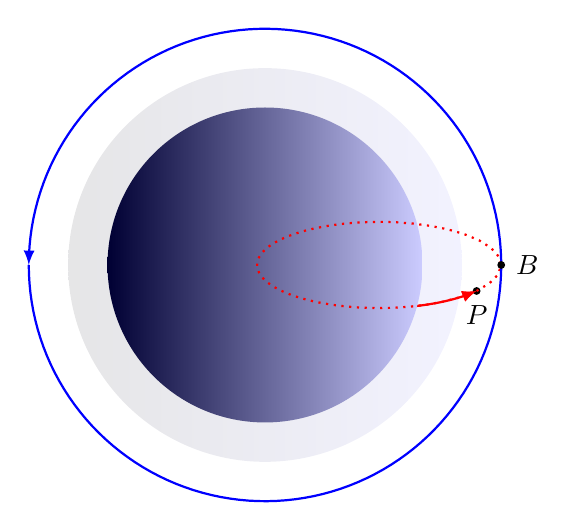
\begin{tikzpicture}
\def\R{2}
\def\h{0.5}
\def\ap{3}
\def\pea{0.1}
\def\peb{3}
\def\an{-7}
\node[loint=O] (O) at (0,0) {};
\path[
	right color=blue!5,
	left color=blue!5!black!10,
]
(O) circle (\R+\h);
\orbit[red]{O}{\ap}{\pea}{-180}{\an};
\path[
	right color=blue!20,
	left color=blue!20!black,
]
(O) circle (\R);
\orbitpoint[boint=P]{O}{\ap}{\pea}{\an}{}{};
\orbit[red,dotted]{O}{\ap}{\pea}{\an}{360+\an};
\orbit[blue]{O}{\ap}{\peb}{-180}{180};
\orbitpoint[roint=B]{O}{\ap}{\peb}{0}{}{};
\end{tikzpicture}
\caption{
	When $\posit{P}$ leaves the atmosphere and burns in $\posit{B}$,
	it can change from the \textcolor{red}{red} “orbit” to the
	\textcolor{blue}{blue} orbit.
}
\end{figure}


\subsection{Classical burn}

Using the \emph{vis-viva} equation~(\ref{eql:visviva}), we can compute
the requisite speed for orbiting:

\[
\speed{v}^2
=
\mathcal G \mass{M} \left(\frac 2 {\dist{r_a}} - \frac 2 {\dist{r_a}+\dist{r_a}}\right)
=
\frac {\mathcal G \mass{M}} {\dist{r_a}}
\]

For example, on Kerbin, you need to reach an horizontal velocity of:

\[
\speed{v_{\text{orbit}}}
=
\sqrt{\frac {6.67 \times 10^{11}~m^3/kg/s^2 \times \mass{5.29 \times 10^{22}~kg}} {\dist{600~km} + \dist{80~km}}}
=
\speed{2279~m/s}
\]

\begin{remark}
To save $\speed{\Delta v}$, launches are done close to the equator to go
with the movement of the surface due to the body's rotation. On Kerbin,
we save ($\delay{T}$ is the orbital period): \[
\speed{v_{\text{surf}}}
=
\frac {2\pi \dist{R}} {\delay{T}}
=
\speed{174.5~m/s}
\]
\end{remark}

\chapter{Maneuvers}
\banner
\chaptquote{xkcd}{
	The six words you \emph{never} say at NASA: “And besides --
	it works in Kerbal Space Program.”
}

The this chapter, we will see how to change from a circular orbit
to another.



\section{Pro-/retro- grade burn}

The vis-viva equation~(\ref{eql:visviva}) tells us:
\[
\speed{v}^2
=
\mathcal G \mass{M} \left(
	\frac 2 {\dist{r}}
	-
	\frac 2 {\dist{r_a} + \dist{r_p}}
\right)
\]

For example, if we are at an apsis (apo- or peri-) and want to rise the
opposite point, we need to speed up (burn prograde), and slow down to
decrease it; the formula above tells us how much so.

\begin{figure}[H]
\centering
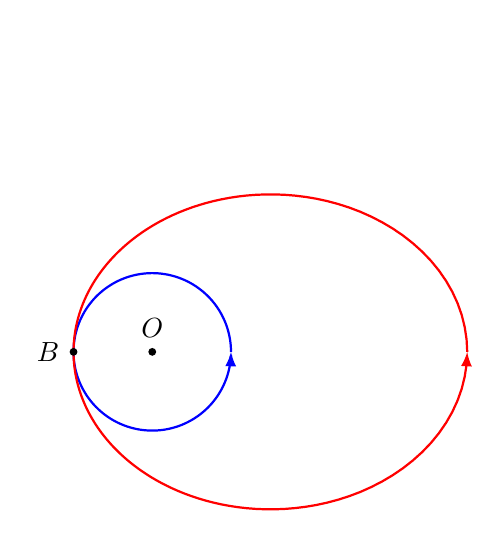
\begin{tikzpicture}
\def\peri{1}
\def\apoa{1}
\def\apob{4}
\node[point=O] (O) at (0,0) {};
\node (A0) at (0,\apoa) {};
\node (A1) at (0,\apob) {};
\orbit[color=blue]{O}{\apoa}{\peri}{0}{360}
\orbit[color=red] {O}{\apob}{\peri}{0}{360}
\node[loint=B] (B) at (-\peri,0) {};
\end{tikzpicture}
\caption{
	A satellite on the \textcolor{blue}{blue} orbit can
	switch to the \textcolor{red}{red} one by burning prograde
	(speeding up) at $\posit{B}$; conversely it can switch from
	the \textcolor{red}{red} orbit to the \textcolor{blue}{blue}
	one by burning retro grade at this same point.
}
\end{figure}

When searching for good trajectories, we are interested in saving
propellant. According to~(\ref{eql:thrust}), this is the same as saving
for $\speed{\Delta v}$ (althgouh proportionally). If $\dist{r}$ is
the apsis where the burn is performed, $\dist{r_0}$ the opposite apsis
before the burn and $\dist{r_1}$ after:
\begin{align*}
\speed{\Delta v}
&=
|\speed{v_1} - \speed{v_0}|
\\
\frac 1 {\sqrt{\mathcal G \mass{M}}} \speed{\Delta v}
&=
\left|
\sqrt{
	\frac 2 {\dist{r}}
	-
	\frac 2 {\dist{r} + \dist{r_1}}
}
-
\sqrt{
	\frac 2 {\dist{r}}
	-
	\frac 2 {\dist{r} + \dist{r_0}}
}
\right|
\eqtag{eql:burn}
\end{align*}



\section{Hohmann transfer}

Now, assume we are in a circular orbit of radius $\dist{r_0}$ and want to
do a simple transfer to a circular orbit of radius $\dist{r_1}$. During
a Hohmann transfer, we first raise our apoapsis to $\dist{r_1}$ and then
the periapsis (from the new apopsis).

\begin{figure}[H]
\centering
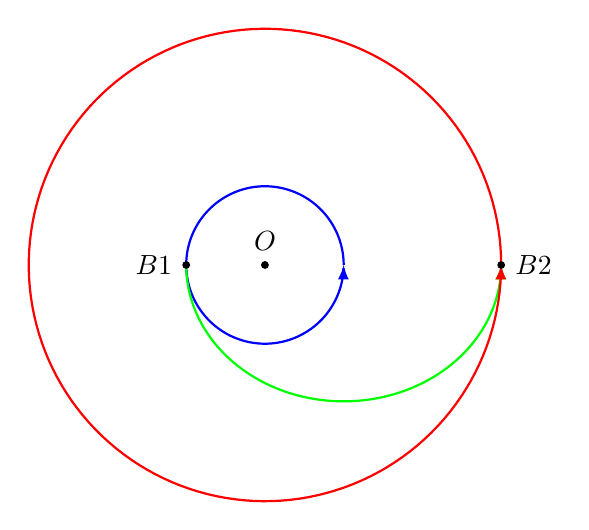
\begin{tikzpicture}
\def\rada{1}
\def\radb{3}
\node[point=O] (O) at (0,0) {};
\orbit[color=blue] {O}{\rada}{\rada}{  0}{360}
\orbit[color=green]{O}{\radb}{\rada}{180}{360}
\orbit[color=red]  {O}{\radb}{\radb}{  0}{360}
\node[loint=B1] (B1) at (-\rada,0) {};
\node[roint=B2] (B2) at ( \radb,0) {};
\end{tikzpicture}
\caption{
	We first switch from the \textcolor{blue}{blue} orbit to the
	\textcolor{green}{green} one by burning at $\posit{B1}$ and then
	from the \textcolor{green}{green} one to the \textcolor{red}{red}
	one by burning at $\posit{B2}$.
}
\end{figure}

\[
\frac 1 {\sqrt{\mathcal G \mass{M}}} \speed{\Delta v}
=
\left|
\sqrt{
	\frac 2 {\dist{r_0}}
	-
	\frac 2 {\dist{r_0} + \dist{r_1}}
}
-
\frac 1 {\sqrt{\dist{r_0}}}
\right|
+
\left|
\frac 1 {\sqrt{\dist{r_1}}}
-
\sqrt{
	\frac 2 {\dist{r_1}}
	-
	\frac 2 {\dist{r_0} + \dist{r_1}}
}
\right|
\]

We can multiply both hands by $\sqrt{\dist{r_0}}$ and set $x = \frac
{\dist{r_1}} {\dist{r_0}}$ to get a simpler expression:

\[
\underbrace{
	\sqrt{\frac {\dist{r_0}} {\mathcal G \mass{M}}}
}_{\alpha}
\speed{\Delta v}
=
\left|
\sqrt{2 - \frac 2 {1 + x}}
-
1
\right|
+
\left|
\frac 1 {\sqrt{x}}
-
\sqrt{\frac 2 x - \frac 2 {1 + x}}
\right|
\]

\begin{figure}[H]
\centering
\begin{tikzpicture}
\begin{axis}[
	samples=\samples,
	domain=0.25:4,
	xtick={0.25,1,2,3,4},
	ytick={0,0.1,0.2,0.3,0.4,0.5,0.6,0.7,0.8,0.9},
	no markers,
	axis lines=left,
	xlabel=$\frac {\dist{r_1}} {\dist{r_0}}$,
	ylabel=$\alpha \speed{\Delta v}$
]
\addplot{abs(sqrt(2-2/(1+x)) - 1) + abs(1/sqrt(x) - sqrt(2/x - 2/(1+x)))};
\end{axis}
\end{tikzpicture}
\caption{
	Note that decreasing an orbit by half costs about as much as the
	converse (doubling it), but dividing it by four costs twice as
	much as the converse.
}
\end{figure}



\section{Bi-elliptical transfer}

The idea is to use three burns instead of two.

\begin{figure}[H]
\centering
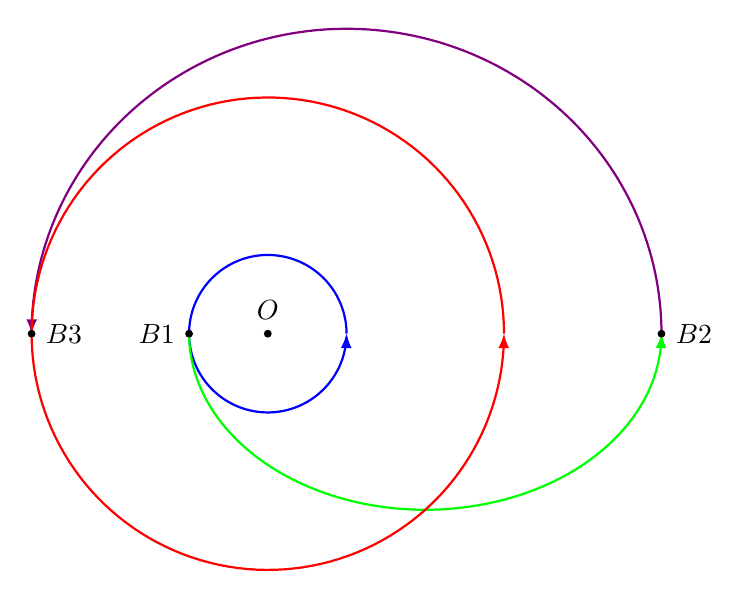
\begin{tikzpicture}
\def\rada{1}
\def\radb{3}
\def\radi{5}
\node[point=O] (O) at (0,0) {};
\orbit[color=blue]  {O}{\rada}{\rada}{  0}{360}
\orbit[color=green] {O}{\radi}{\rada}{180}{360}
\orbit[color=violet]{O}{\radi}{\radb}{  0}{180}
\orbit[color=red]   {O}{\radb}{\radb}{  0}{360}
\node[loint=B1] (B1) at (-\rada,0) {};
\node[roint=B2] (B2) at ( \radi,0) {};
\node[roint=B3] (B3) at (-\radb,0) {};
\end{tikzpicture}
\caption{
	During a bi-elliptical transfer, we use two intermediate orbits
	(\textcolor{green}{green}, then \textcolor{violet}{violet});
	the idea is that it will be easier to raise the
	\textcolor{green}{green} periapsis from a higher apoapsis
}
\end{figure}

\begin{align*}
\frac 1 {\sqrt{\mathcal G \mass{M}}} \speed{\Delta v}
=&
\left|
\sqrt{
	\frac 2 {\dist{r_0}}
	-
	\frac 2 {\dist{r_0} + \dist{r_1}}
}
-
\frac 1 {\sqrt{\dist{r_0}}}
\right|
\\
&+
\left|
\sqrt{
	\frac 2 {\dist{r_1}}
	-
	\frac 2 {\dist{r_2} + \dist{r_1}}
}
-
\sqrt{
	\frac 2 {\dist{r_1}}
	-
	\frac 2 {\dist{r_0} + \dist{r_1}}
}
\right|
\\
&+
\left|
\frac 1 {\sqrt{\dist{r_2}}}
-
\sqrt{
	\frac 2 {\dist{r_2}}
	-
	\frac 2 {\dist{r_2} + \dist{r_1}}
}
\right|
\end{align*}

Again, we set $x = \frac {\dist{r_2}} {\dist{r_0}}$ and $y = \frac
{\dist{r_1}} {\dist{r_0}}$ and:
\begin{align*}
\underbrace{
	\sqrt{\frac {\dist{r_0}} {\mathcal G \mass{M}}}
}_{\alpha}
\speed{\Delta v}
=&
\left|
\sqrt{2 - \frac 2 {1 + y}}
-
1
\right|
\\
&+
\left|
\sqrt{\frac 2 y - \frac 2 {x + y}}
-
\sqrt{\frac 2 y - \frac 2 {1 + y}}
\right|
\\
&+
\left|
\frac 1 {\sqrt{x}}
-
\sqrt{\frac 2 x - \frac 2 {x + y}}
\right|
\end{align*}

\begin{figure}[H]
\centering
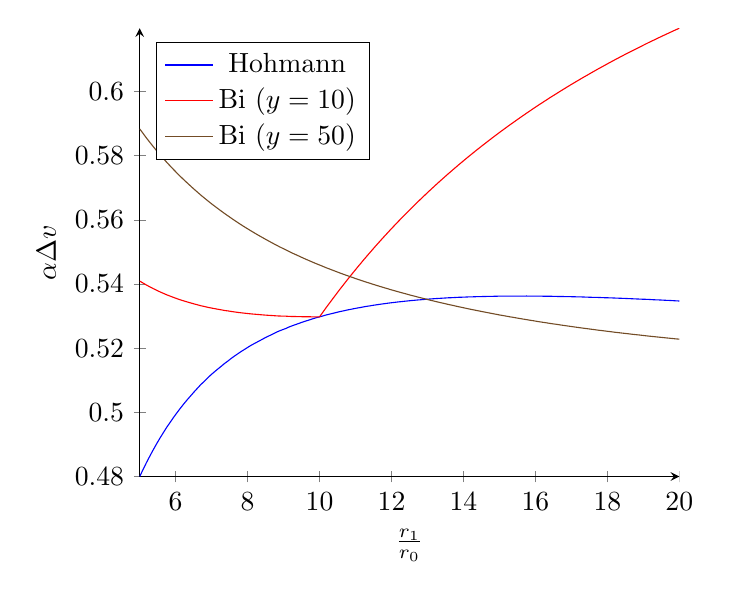
\begin{tikzpicture}
\begin{axis}[
	samples=\samples,
	domain=5:20,
	no markers,
	axis lines=left,
	xlabel=$\frac {\dist{r_1}} {\dist{r_0}}$,
	ylabel=$\alpha \speed{\Delta v}$,
	legend pos=north west,
]
\addplot{abs(sqrt(2-2/(1+x)) - 1) + abs(1/sqrt(x) - sqrt(2/x - 2/(1+x)))};
\addlegendentry{Hohmann}
\foreach \myy in {10,50}{
	\addplot{abs(sqrt(2-2/(1+\myy)) - 1) + abs(sqrt(2/\myy - 2/(x+\myy)) - sqrt(2/\myy - 2/(1+\myy))) + abs(1/sqrt(x) - sqrt(2/x - 2/(x+\myy)))};
	\edef\temp{\noexpand
	\addlegendentry{Bi ($y = \myy$)}
	}\temp
}
\end{axis}
\end{tikzpicture}
\end{figure}

\clearpage



\section{Inclination change}

\begin{important}
Remember, we are only considering \textbf{circular} orbits. The formulas
and derivations below only make sense for circular orbits. We advise
you to set your inclination in a circular orbit before any subsequent
maneuver.
\end{important}


\subsection{(Anti-)normal burn}

Consider the orbital plane in which a satellite is moving. We are
interested in the effect of an acceleration orthogonal to the plane
(normal or antinormal). For this, we study the evolution of the velocity.

\begin{figure}[H]
\centering
\begin{tikzpicture}[->,thick]
\node[boint=P] (P)   at (0,0) {};
\node (V)   at ( 50:3)    {$\speed{\overrightarrow v}$};
\node (dV)  at (140:1)    {$\speed{\overrightarrow {\d v}}$};
\node (VdV) at ($(V)+(dV)$) {$\speed{\overrightarrow {v + \d v}}$};
\draw[->,thick] (P) -- (V);
\draw[->,thick] (P) -- (dV);
\draw[->,thick] (P) -- (VdV);
\markangle{V}{P}{VdV}{$\d \theta$}{1.5}
\end{tikzpicture}
\caption{
	The satellite is heading towards $\speed{\vec v}$ and an
	acceleration is applied to it so that during a time $\delay{\dt}$,
	its velocity is changed by $\speed{\vec{\d v}}$.
}
\label{fig:normalburn}
\end{figure}

As seen in figure~(\ref{fig:normalburn}), we can easily find the change
in inclination:
\begin{align*}
\angle{\d \theta}
\simeq
\tan \angle{\d \theta}
&=
\frac {\speed{\d v}} {\speed{v}}
\\
\int \frac {\angle{\d \theta}} {\delay{\dt}} \delay{\dt}
&=
\int \frac {\accel{a} \delay{\dt}} {\speed{v}}
\\
\angle{\theta}
&=
\frac {\accel{a} \delay{t}} {\speed{v}}
=
\frac {\speed{\Delta v}} {\speed{v}}
\end{align*}


\subsection{Straight burn}

Doing a $180^{\circ}$ inclination chage using a constant radial burn like
exposed above yields a $\speed{\Delta v}$ proportional to the current
orbital velocity $\speed{v}$: $\speed{\Delta v} = \angle{\pi} \speed{v}
\simeq 3 \speed{v}$. However, simply going retrograde until the speed is
reverse only yields $\speed{\Delta v} = 2 \speed{v}$ for the same result.

You can find another derivation of the cost in \cite[page
2]{incproof,incproof2}.

\begin{figure}[H]
\centering
\begin{tikzpicture}[->,thick]
\node[boint=P] (P)   at (0,0) {};
\coordinate (V0) at (40:3);
\coordinate (V1) at (80:3);
\coordinate (VV) at ($(V1)-(V0)$);
\draw (P) -- +(V0) node[above]{$\speed{\overrightarrow {v_0}}$};
\draw (P) -- +(V1) node[above]{$\speed{\overrightarrow {v_1}}$};
\draw[red] (P) -- +(VV) node[above]{$\speed{\overrightarrow {\Delta v}}$};
\draw[red] (V0) -- +(VV);
\markangle{V0}{P}{V1}{$\theta$}{1}
\end{tikzpicture}
\caption{
	A rotation of angle $\angle{\theta}$ from velocity vector
	$\speed{\vec{v_0}}$ to $\speed{\vec{v_1}}$ is done in a straight
	change in speed $\speed{\Delta v}$.
}
\end{figure}

We need to compute $\speed{\Delta v}$ for given $\speed{v} =
\speed{|\vec{v_0}|} = \speed{|\vec{v_1}|}$ and $\angle{\theta}$. Because
the triangle is isosceles, the altitude and the median from $P$ are
one so:
\[
\speed{\Delta v}
=
\left|2 \speed{v} \sin \frac {\angle{\theta}} 2\right|
\]

For $\angle{\theta} = \angle{\pi}$, we get $\speed{\Delta v} = 2
\speed{v}$ which is the expected result.

\begin{figure}[H]
\centering
\begin{tikzpicture}
\begin{axis}[
	samples=\samples,
	domain=-180:180,
	xtick={-180,-135,...,180},
	no markers,
	axis lines=left,
	xlabel=$\theta$ ($^{\circ}$),
	ylabel=$\frac {\speed{\Delta v}} {\speed{v}}$,
]
\addplot{abs(2*sin(x/2))};
\end{axis}
\end{tikzpicture}
\caption{
	An inclination change of about $\angle{30^{\circ}}$ already costs
	half the orbital speed; $\angle{60^{\circ}}$ costs as much as
	the orbital speed.
}
\end{figure}


\subsection{Bi-elliptical inclination change}

Whatever the method used for the inclination change, the cost is
proportional to the current orbital speed. Thus, it is more efficient to
do such a maneuver at low speed (e.g. at apoapsis). /u/ObsessedWithKSP
demonstrated a maneuver similar to the bi-elliptical transfer for a more
efficient plane change \cite{biincchange,biincchange2}.

A formal derivation of the optimal inclination change has been published
by /u/listens\_to\_galaxies \cite{incproof,incproof2}.

\begin{figure}[H]
\centering
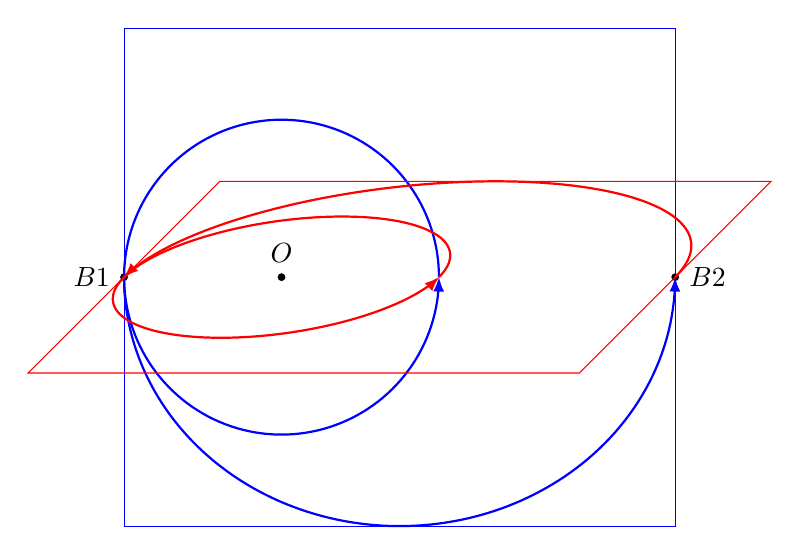
\begin{tikzpicture}
\def\rada{2}
\def\radi{5}
\def\width{\rada^0.5 * \radi^0.5}
\node[point=O] (O) at (0,0) {};
\node[loint=B1] (B1) at (-\rada,0) {};
\node[roint=B2] (B2) at ( \radi,0) {};
\begin{scope}[canvas is xy plane at z=0,color=blue]
\orbit{O}{\rada}{\rada}{0}{360}
\orbit{O}{\radi}{\rada}{180}{360}
\draw (-\rada,-\width) rectangle (\radi,\width);
\end{scope}
\begin{scope}[canvas is zx plane at y=0,rotate=90,color=red]
\draw (-\rada,-\width) rectangle (\radi,\width);
\orbit{O}{\radi}{\rada}{0}{180}
\orbit{O}{\rada}{\rada}{0}{360}
\end{scope}
\end{tikzpicture}
\caption{
	Starting in the \textcolor{blue}{blue} plane on the circular
	orbit, the spacecraft first burns prograde in $\posit{B1}$
	to raise its apoapsis to $\posit{B2}$; once there, its speed
	is lower and it can proceed to the inclination change to
	the \textcolor{red}{red} plane effectively; finaly, it burns
	retrograde back in $\posit{B1}$ to return to a circular orbit.
}
\end{figure}



\section{Radial in/out burn}



\section{Arbitrary burn}

\include{operating}
\renewcommand{\cleardoublepage}{\ifodd\thepage\null\newpage\fi}
\fancyhf{}
\renewcommand{\footrulewidth}{0pt}
\begin{thebibliography}{99}
\ClearWallPaper

\bibitem{ksp}
“Kerbal Space Program”, \\
2011--2014, early access game, Squad, \\
\url{https://www.kerbalspaceprogram.com/}

\bibitem{threekerbalmun}
“Three Kerbal Mun” \\
2011, deviantART publication, MK01, \\
\url{https://mk01.deviantart.com/art/Three-Kerbal-Mun-272960572}

\bibitem{banners}
“Renderings of my favourite planets/muns in banner form”, \\
2013, KSP forum post, Lunniy Korabl, \\
\url{http://forum.kerbalspaceprogram.com/threads/34329}

\bibitem{revxkcd}
“The Six Words You Never Say in KSP”, \\
2013, KSP forum post, Hayoo, \\
{\footnotesize \url{http://forum.kerbalspaceprogram.com/threads/50660?p=764793#post764793}}

\bibitem{rareden}
“Rareden's Projects”, \\
2013, KSP forum post, Rareden, \\
\url{http://forum.kerbalspaceprogram.com/threads/25231}

\bibitem{biincchange}
“How to do a bi-elliptic inclination change transfer orbit in one picture.”,
2014, Reddit submission, /u/ObsessedWithKSP, \\
\url{https://pay.reddit.com/r/KerbalSpaceProgram/comments/23ri7a}

\bibitem{biincchange2}
“How to do a bi-elliptic inclination change transfer orbit in one picture.”,
2014, Reddit submission, /u/ObsessedWithKSP, \\
\url{https://pay.reddit.com/r/KerbalSpaceProgram/comments/23ri7a}

\bibitem{incproof}
“[D]erivation of the [optimal] inclination change transfer orbit”, \\
2014, Reddit submission, /u/listens\_to\_galaxies, \\
\url{https://pay.reddit.com/r/KerbalAcademy/comments/23v5wo}

\bibitem{incproof2}
“Bi-elliptic inclination change transfer orbit”, \\
2014, imgur album, /u/listens\_to\_galaxies, \\
\url{https://imgur.com/a/uM7PK}

\bibitem{rt2}
“Tutorial: Complete Novice's Guide to RemoteTech 2”, \\
2013, Reddit submission, /u/Grays42, \\
\url{https://pay.reddit.com/r/KerbalSpaceProgram/comments/1rml0r}

\bibitem{coverage}
“Tutorial: Satellite Coverage”, \\
2013--2014, KSP wiki article, XZise \emph{et alii}, \\
{\small\url{http://wiki.kerbalspaceprogram.com/wiki/Tutorial:Satellite_Coverage}}

\bibitem{gwells}
“Kerbal Gravity Wells”, \\
2013, Reddit submission, /u/jofwu, \\
\url{https://pay.reddit.com/r/KerbalSpaceProgram/comments/1o3epz}

\bibitem{xkcd1244}
“Six Words”, \\
2013, webcomic, xkcd, \\
\url{https://xkcd.com/1244/}

\bibitem{xkcd1356}
“Orbital Mechanics”, \\
2014, webcomic, xkcd, \\
\url{https://xkcd.com/1356/}

\bibitem{flags}
“KSP -- Flags”, \\
2013, Imgur album, /u/shard013, \\
\url{https://imgur.com/a/rRUZp}

\bibitem{voyagerassists}
“Ken Lunn's Voyager Spacecraft Page”, \\
2012, web page, Ken Lunn, \\
\url{http://usuaris.tinet.org/klunn/voyager.html}

\bibitem{cassiniassists}
“Cassini interplanetary trajectory”, \\
2006, SVG diagram, User:Pline, \\
{\footnotesize\url{https://en.wikipedia.org/wiki/File:Cassini_interplanet_trajectory.svg}}

%\bibitem{scottmanley}
%“Scott Manley”, \\
%2009--2014, Youtube channel, Scott Manley, \\
%\url{https://www.youtube.com/user/szyzyg}

\ThisLLCornerWallPaper{1}{img/spaceKerbal_1920x1080.png}
\end{thebibliography}

\pagecolor{black}
\color{black!30}

\ifodd\thepage\null\newpage\fi

\vspace*{\fill}
\chaptquote{Stephen Hawking}{
	My goal is simple. It is a complete understanding of the universe,
	why it is as it is and why it exists at all.
}

\end{document}
